
\begin{question}
Please make a frequency table and a bar chart from the following
(unsorted) discrete data.

\begin{longtable}[]{@{}rrrrr@{}}
\toprule
\endhead
9 & 6 & 3 & 9 & 4\tabularnewline
6 & 8 & 6 & 9 & 5\tabularnewline
11 & 11 & 10 & 10 & 10\tabularnewline
9 & 7 & 10 & 10 & 6\tabularnewline
\bottomrule
\end{longtable}
\end{question}

\begin{solution}
Make a frequency table.

\begin{longtable}[]{@{}rr@{}}
\toprule
value & frequency\tabularnewline
\midrule
\endhead
3 & 1\tabularnewline
4 & 1\tabularnewline
5 & 1\tabularnewline
6 & 4\tabularnewline
7 & 1\tabularnewline
8 & 1\tabularnewline
9 & 4\tabularnewline
10 & 5\tabularnewline
11 & 2\tabularnewline
\bottomrule
\end{longtable}

Make the bar chart.

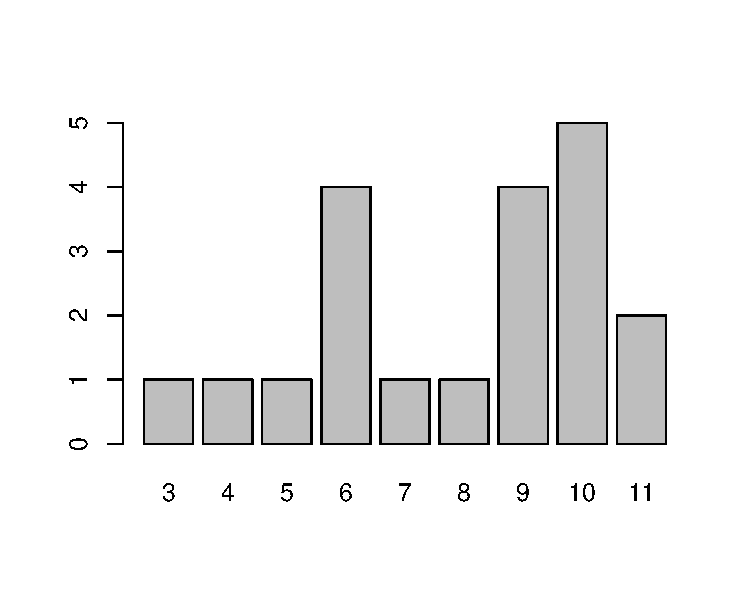
\includegraphics{barchart-1-3.pdf}\\
\end{solution}

